\documentclass[11pt]{article}
 
\usepackage[margin=1in]{geometry} 
\usepackage{amsmath,amsthm,amssymb}
\usepackage{enumitem, graphicx, float, caption}
\usepackage{amsmath}
\usepackage{bm}
\usepackage{tikz}
\usepackage{listings}
\usetikzlibrary{arrows.meta}
 

 
\begin{document}
 

 
\title{Midterm 1}
%%%%%%%%%%%%%%%%%%%%%%%%%%%%%%%%%%%%%%%%%%%%%%%
%Change your name
%%%%%%%%%%%%%%%%%%%%%%%%%%%%%%%%%%%%%%%%%%%%%%%
\author{Your Name \\ 
MATH 87 Math Modeling} 

\maketitle
%%%%%%%%%%%%%%%%%%%%%%%%%%%%%%%%%%%%%%%%%%%%%%%%%%%%%%%%%%%%%%%%%%%%%%%%%%%%%%%%%%
This should be typed as a report, but I'll put some useful things in here for you to consider.

\section{Here's how you make a section}
\section{Introduction}
\subsection{Here's how you make a subsection}




here's one way to make a network diagram, but tikz can be tricky, so you don't have to do it this way.

\begin{figure}[H]
\begin{center}
%change scale to change the size of your figure and get it to fit on the page
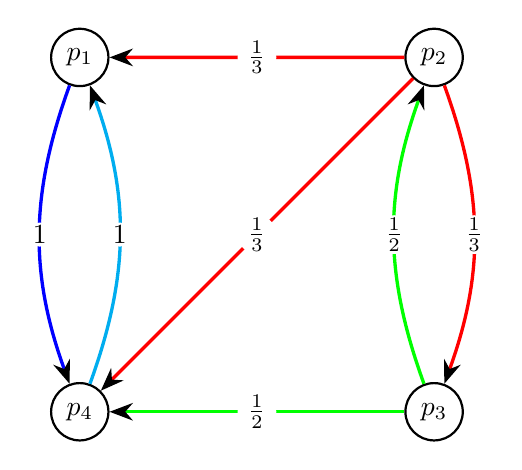
\begin{tikzpicture}[scale = 1.5]
\begin{scope}[every node/.style={circle,thick,draw}]
	%this numbers nodes (1-4 here), draws them at a certain coordinate, and gives them a label
	%don't forget semicolons at the end!!!
    \node (4) at (0,0) {$p_4$};
    \node (1) at (0,3) {$p_1$};
    \node (2) at (3,3) {$p_2$};
    \node (3) at (3,0) {$p_3$};
\end{scope}



%this part is how you draw edges with edge weights on them, and do things like curve the edges and change the colors


%all of the red edges. Change the draw=red to change the color
\begin{scope}[>={Stealth[black]},
              every node/.style={fill=white,circle, inner sep=.2pt,minimum size=.5pt},
              every edge/.style={draw=red,very thick}]
              
    %draws edge from node 2 to node 1 with edge label 1/3
    \path [->] (2) edge node{$\frac{1}{3}$} (1);
    %draws bendy edge from node 2 to node 3 with edge label 1/3
    \path [->] (2) edge[bend left=20] node{$\frac{1}{3}$} (3);
    %draws edge from node 2 to node 4 with edge label 1/3
    \path [->] (2) edge node{$\frac{1}{3}$} (4);
\end{scope}


%same idea, but with blue edges
\begin{scope}[>={Stealth[black]},
              every node/.style={fill=white,circle, inner sep=.2pt,minimum size=0pt},
              every edge/.style={draw=blue,very thick}]
    \path [->] (1) edge[bend right = 20] node{$1$} (4);
\end{scope}

%same idea, but with green edges
\begin{scope}[>={Stealth[black]},
              every node/.style={fill=white,circle,inner sep=.2pt,minimum size=.5pt},
              every edge/.style={draw=green,very thick}]
    \path [->] (3) edge[bend left=20] node{$\frac{1}{2}$} (2);
    \path [->] (3) edge node{$\frac{1}{2}$} (4);
\end{scope}

%same idea, but with light blue edges
\begin{scope}[>={Stealth[black]},
              every node/.style={fill=white,circle,inner sep=.2pt,minimum size=.5pt},
              every edge/.style={draw=cyan,very thick}]
    \path [->] (4) edge[bend right=20] node{$1$} (1);
\end{scope}
\end{tikzpicture}
\caption{caption for the diagram}
\end{center}
\end{figure}

%insert your figure like this if you don't use tikz
%\begin{figure}[H]
%\begin{center}
%change the file name to your file and change the scale number to make it the right size
%\includegraphics[scale=3]{filename}
%\end{center}
%\caption{your caption!}
%\end{figure}



Here's how you make a matrix
\begin{equation*}
T = \begin{bmatrix}
0 & {\frac{1}{3}} & 0 & {1} \\
0 & 0 & {\frac{1}{2}}& 0 \\
0 &{\frac{1}{3}} & 0 & 0 \\
{1} &{\frac{1}{3}} & {\frac{1}{2}} & 0
\end{bmatrix}
\end{equation*}

You an write a linear program like this
\begin{align*}
 \operatorname{max} f(x,y) = your function & \text{\quad s.t.} \\
constraint 1  &\leq  value 1 \\
constraint 2 &\leq value 2 \\
constraint 3 &\leq value 3 
\end{align*}

\begin{table}[H]
\begin{center}
%add more columns by adding more |c| below
\begin{tabular}{|c|c|c|c|c|}
\hline 
• & • & • & • & • \\ 
\hline 
• & • & • & • & • \\ 
\hline 
• & • & • & • & • \\ 
\hline 
• & • & • & • & • \\ 
\hline 
• & • & • & • & • \\ 
\hline 
• & • & • & • & • \\ 
\hline 

%add more rows by adding this \\ \hline 
% \\ adds more rows, use & to separate entries in columns
\end{tabular} 
\caption{Caption for the table}
\end{center}
\end{table}

This is how you include the code:
\begin{lstlisting}
include numpy as np

a=b
\end{lstlisting}

\end{document}